\section{Introduction}
%%% TODO: add motiviation for cell diffusion models from real world applications 
% from bridge paper:
- Collective cell migration is a key driver of embryonic development, wound healing, and some types of cancer invasion
- It has long been recognized that cells move as collectives during development, regeneration, and wound healing.
Reports from the late nineteenth century already agreed that these processes involve collective movements of cells but mechanisms remained controversial~\cite{alert2020, holmes1914, herrick1932, vaughan1966}
- cell movements were driven by pressure, either preexisting in the tissue or generated de novo by cell division~\cite{herrick1932}. 
- Others claimed that cells would move by spreading their volume to occupy the largest possible surface~\cite{alert2020}.
- Still others defended that cell sheets advanced by the active pulling force generated by leader cells at the tissue margin~\cite{holmes1914}
- Later, the discovery of genes and proteins shifted the attention from the whole to the parts, and the search for a global physical understanding of collective migration was largely abandoned
- This trend has been reversed in the last decade due to groundbreaking technical~\cite{roca2017} and conceptual~\cite{marchetti2013, prost2015, julicher2018} advances together with a progressive questioning of reductionist approaches~\cite{good2018}.
- Furthermore, a range of new technologies such as traction microscopy have enabled the direct mapping of the forces that cells exert on their surroundings as they migrate~\cite{du2005, trepat2009}. All mechanical variables relevant to the problem of collective cell migration have thus become available in time and space
- Finally, life scientists have recognized that collective cell migration is not only key to development, regeneration, and wound healing but also to devastating diseases such as cancer~\cite{friedl1995}.
- The coincidence in time of these different technological and conceptual advances has placed collective cell migration back at the center of research at the interface between life and physical sciences.
- Collective cell migration comes in different flavors depending on the biological tissue and process~\cite{friedl2009}.
- During epithelial morphogenesis, wound healing, and regeneration, cells generally move as sheets adhered on an inert hydrogel called the extracellular matrix (ECM). In some forms of cancer invasion, cells also invade as sheets at the interface between tissues 
- both in development and in tumor invasion, cells invade as strands or clusters within a complex three-dimensional environment composed of ECM and different cell types~\cite{friedl2009, cai2014, clark2015} 
- we remain far from accessing physical forces in three dimensions (3D), so we focus this review on cell sheets migrating in two dimensions
% from axel wenzel 
- Confluent cell monolayers and epithelia tissues show remarkable patterns and correlations in structural arrangements and actively driven collective flows~\cite{wenzel2021}
- To identify the principles that govern collective cell migration in such systems has seen a growing interest in recent years. Experimental investigations on cell monolayers and epithelial tissue of model systems have shown remarkable patterns and correlations in cell migration. These include an unjamming transition between a glassy phase and a fluid phase the spontaneous formation of vortices and topological defects, as well as the emergence of active turbulent flows
- A fundamental challenge is to understand how this macroscopic behavior is linked to the properties of individual cells and physical cell-cell interactions, which is the target of a large variety of modeling approaches. These approaches differ by the level of coarsegraining and range from subcellular lattice models and multiphase field models, to vertex and Voronoi models, particle models, and continuum models on a multicellular scale 
- The systematic comparison of cell models will hopefully help to select the appropriate approach in future studies and provide a route towards predictive simulations of patterns and correlations in cell colonies.

% intro pp model 
We consider the point particle model on a two dimensional bounded domain $\Omega \subset \mathbb{R}^2$, where we have $N \in \N$ particles and have no real size.
There is also no particle interaction, as there is no possibility of collision. 
Initially, the particles are randomly distributed in $\Omega$. \\
The particles' dynamics are governed solely by Brownian motion.
Brownian motion is a random and unpredictable motion that occurs in the real world when particles are suspended in a fluid and collide with surrounding molecules. \\
In mathematics, we model Brownian motion using stochastic differential equations (SDEs), which are equations that describe the motion of a particle over time in a random and unpredictable manner. 
SDEs are a powerful tool for modeling complex phenomena in physics, finance, and other fields, and are characterized by the presence of random terms that capture the uncertainty of the system. \\
Let 
\[\vec{x}_i(t) \in \Omega \quad 1 \leq i \leq N,\]
be the location of the particle $i$ at time $t > 0$. 
The particle movement can be modeled using the diffusion equation, which describes the random motion of particles over time
\begin{center}
	$d\vec{x}_i(t) = \sqrt{2D} \: dB_t^{(i)}, \quad 1 \leq i \leq N$,
\end{center}
where the constant $D > 0$ represents the diffusion coefficient which proportionally scales the speed of the particle movements by scaling the random fluctuations.
The term $dB_t^{(i)}$ introduces the randomness of Brownian motion, where $dB_t^{(i)}$ is a normally distributed random variable that accounts for the unpredictable changes in the position of particle $vec{x}_i$ over time. \\
We also consider the probability density function $\rho(t, \vec{x})$, which describes the probability of finding a particle at a specific position $\vec{x}$ at time $t$.
In the given context, the function $\rho$ satisfies the partial differential equation:
\begin{align}
	\dfrac{\partial \rho (t, \vec{x})}{\partial t} = D \Delta_{\vec{x}} \rho(t, \vec{x}) \label{eq:pointparticle}, 
\end{align}
where $\Delta_{\vec{x}}$ is the Laplacian operator with respect to the spatial variables. \\
Equation~\eqref{eq:pointparticle} represents the classic diffusion equation, a cornerstone of physics and mathematics.
The same diffusion constant $D>0$ is used in the SDE for particle movement and the PDE for the probability density function $\rho$. \\



% intro hp model 
\textbf{Hard sphere model} \\
Next, we consider models that add a real size to the particles and introduce particle interactions. 
With the inclusion of a real size, the particles cannot overlap, resulting in exclusion effects. 
To account for this, we introduce a new interaction dynamics that ensures the particles do not overlap. 
This new interaction dynamics leads to a more complex and realistic model that captures the behavior of particles with a real size and interactions. \\
Since particles cannot overlap, the domain $\Omega^{(i)}_{\epsilon}$, that holds the information where the centre of particle $i$ can be located, must exclude the areas where $\norm[\vec{x}_i - \vec{x}_j] \leq \epsilon$ for all $1 \leq j \leq N,$ $j \neq i$. 
This is due to the fact that particles cannot occupy the same space simultaneously. \\
The domain that holds all possible locations of the particles is then given by \[\Omega^N_{\epsilon} = \Omega^{(1)}_{\epsilon} \times \ldots \times \Omega^{(N)}_{\epsilon} .\] 
This can be visualized as a product space, where each particle's domain is combined to form a larger domain that encompasses all possible locations of the particles.
Under this circumstances, we will get a new dynamic compared to the point particle model.  \\
In the work of Bruna et al.~\cite{Bruna2012}, a hard sphere particle model is examined.
Here, the particles are spherical in shape, with a diameter $0 < \epsilon \ll 1$.
All particles in this model are distinct and can be distinguished from one another. \\
The hard sphere model is characterized by the fact that any interaction between particles may cause a change in their direction of motion, but the spherical shape of the particles remains unchanged.
Hardcore collisions are modeled as reflective boundary conditions on the collision surfaces defined by $r = \norm[\vec{x}_i - \vec{x}_j] = \epsilon$, where $1 \leq i < j \leq N$.
The external forces acting on a particle in the system are described by the force function $f: \R^2 \rightarrow \R^2$, which depends only on the location of the particle.
The function $\vec{F}$ maps the particle configuration $\vec{X} = (\vec{x}_1, \ldots, \vec{x}_N)^T$ to the vector of external forces $\vec{F}(\vec{X}) = (f(\vec{x}_1), \ldots, f(\vec{x}_N))^T$.
The dynamics of the particles are governed by the SDE
\begin{center}
	$d\vec{x}_i(t) = \sqrt{2D} \: dB_t^{(i)} + f(\vec{x}_i(t)) \: dt, \qquad 1 \leq i \leq N$.
\end{center}
In this model, the particles are initially randomly distributed in $\Omega^N_{\epsilon}$, ensuring that no overlap occurs between the particles.
The joint probability density function $P$ of the $N$ particles satisfies the high-dimensional Fokker-Planck equation
\begin{center}
	$\dfrac{\partial P}{\partial t} = \nabla_{\vec{X}} \cdot (D \nabla_{\vec{X}} P - P \vec{F})$,
\end{center}
where $\nabla_{\vec{X}}$ and $\nabla_{\vec{X}} \cdot$ denote the gradient and divergence operators with respect to the $N$-particle position vector $\vec{X}$.\\
Using the method of matched asymptotic expansions, the authors also derived the probability density function $\rho$ of finding a single particle at time $t$ and position $\vec{x}$, which satisfies the equation
\begin{align}
	\dfrac{\partial \rho (t, \vec{x})}{\partial t} = \Delta_{\vec{x}} \rho + \alpha_d (N - 1) \epsilon^d \Delta_{\vec{x}} (\rho^2) - \nabla_{\vec{x}} \cdot (f(\vec{x}) \rho).
\end{align}
When $f$ is neglected and $\epsilon \rightarrow 0$, this equation reduces to the probability density function of the point particle model, except for a rescaling factor.
Similarly, the Fokker-Planck equation is a direct extension of the diffusion equation, with an additional drift term.\\



% bachelor intro sp model 
\textbf{Soft sphere model} \\
Next, we consider an extension of the model by introducing deformable soft spherical particles. 
This new model incorporates the effect of deformation and interaction between particles through a potential energy function that depends on the distance between the particles.
The paper~\cite{Bruna2017}, written by Bruna, Chapman and Robinson, analyses the diffusion properties of such a model. \\
The equation of motion for each particle $i$ is given by
\begin{equation}
d\vec{x}_i(t) = \sqrt{2D} \: dB_t^{(i)} + f(\vec{x}_i(t))\: dt - \sum\limits_{j\neq i} \nabla_{\vec{x}_i} u (\norm[ \vec{x}_i(t) - \vec{x}_j(t)]) \: dt, \qquad 1 \leq i \leq N,
\end{equation}
where $\nabla_{\vec{x}_i}$ is the gradient with respect to $\vec{x}_i$. \\
The effect of the interaction potential is to cause particles to repel or attract each other depending on the distance between them, rather than simply overlapping. \\
For the modeling of short range interacting soft sphere particles, the authors computed the one particle probability density $\rho(t, \vec{x})$ of finding a given particle at position $\vec{x}$ at time $t$ developing according to
\begin{equation}
\dfrac{\partial \rho}{\partial t} = \nabla_{\vec{x}} \cdot (D \nabla_{\vec{x}} \rho - f(\vec{x}) \rho + \alpha_u \epsilon_u^2(N-1)\rho \nabla_{\vec{x}} \rho)
\end{equation}
where $\alpha_u$ depends on the interaction potential $u$ and $0 < \epsilon_u \ll 1$ is the interaction range of $u$.


%figure for point particles, hard and soft sphere particles, phase field and vertex model
\begin{figure}[t!]
	\centering
	\begin{subfigure}{0.4\textwidth}
		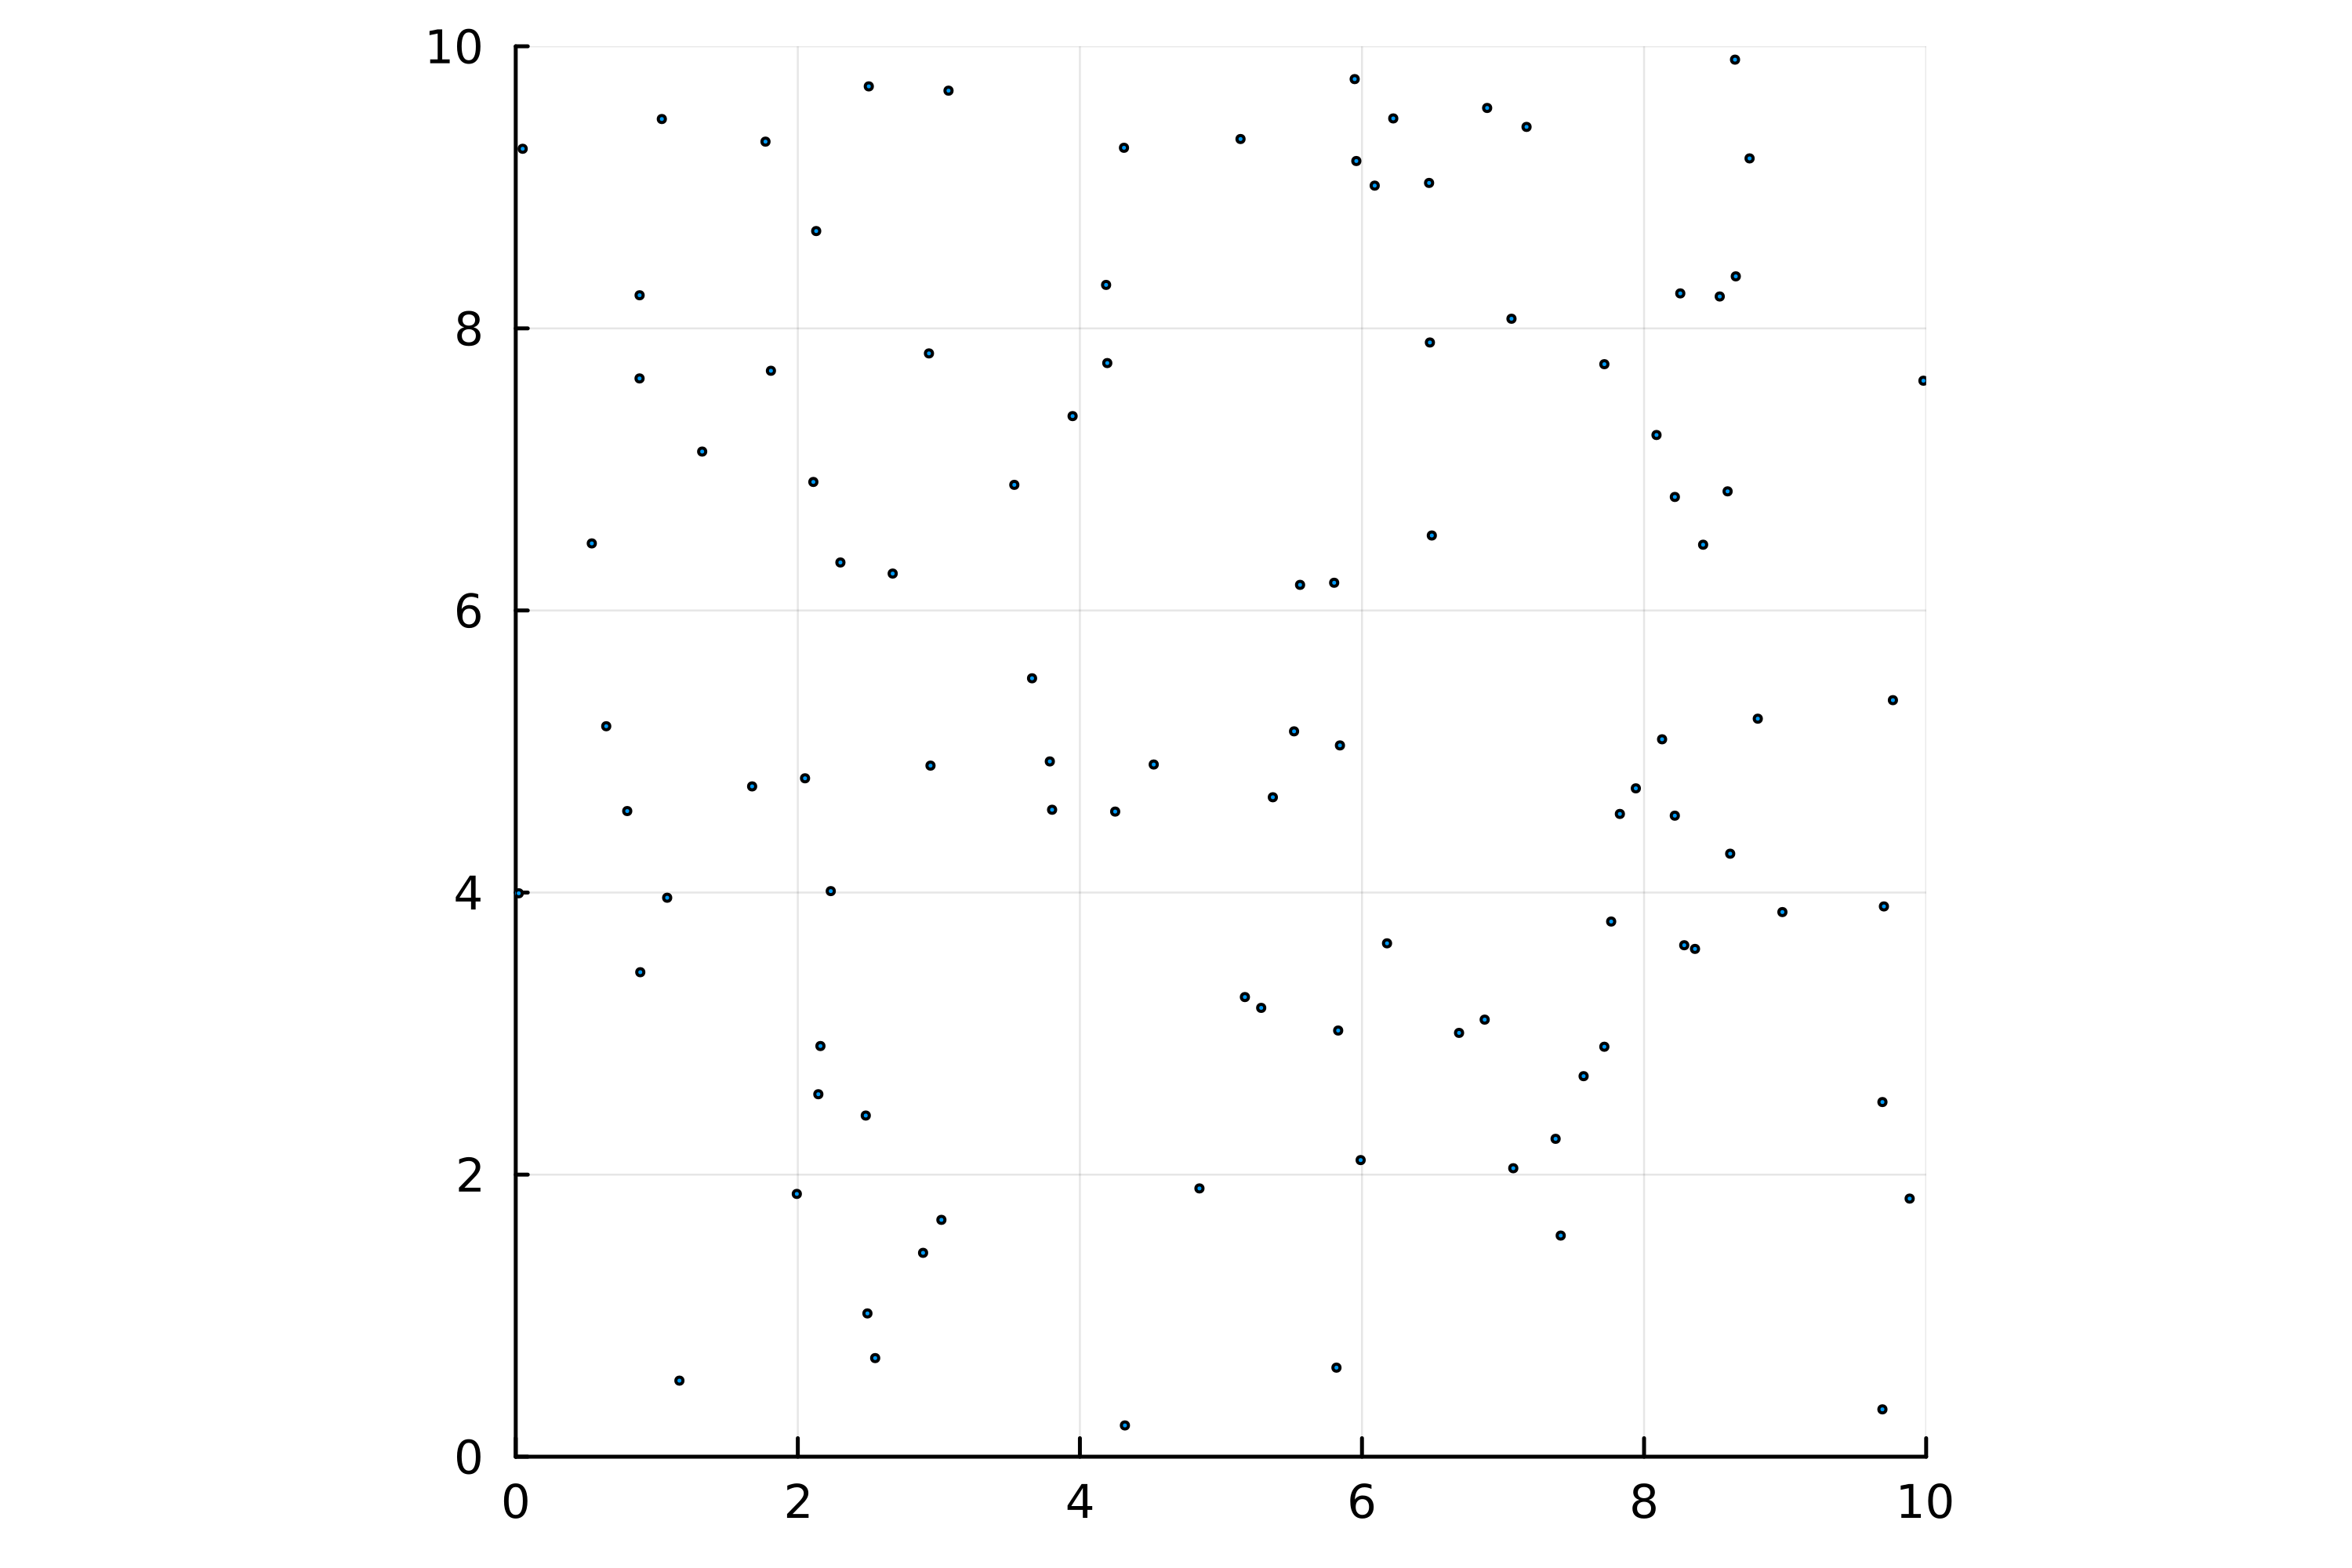
\includegraphics[width=\textwidth]{bachelors-thesis/model_illustrations/particleModel.png}
		\caption{Here, one can see a possible snapshot of the point particle model that is explained at the beginning. 
        The particles are randomly distributed in $\Omega$. 
        The execution of the Brownian motion will cause the particle density to change according to the Diffusion equation.}
	\end{subfigure}
	\hfill
	\begin{subfigure}{0.4\textwidth}
		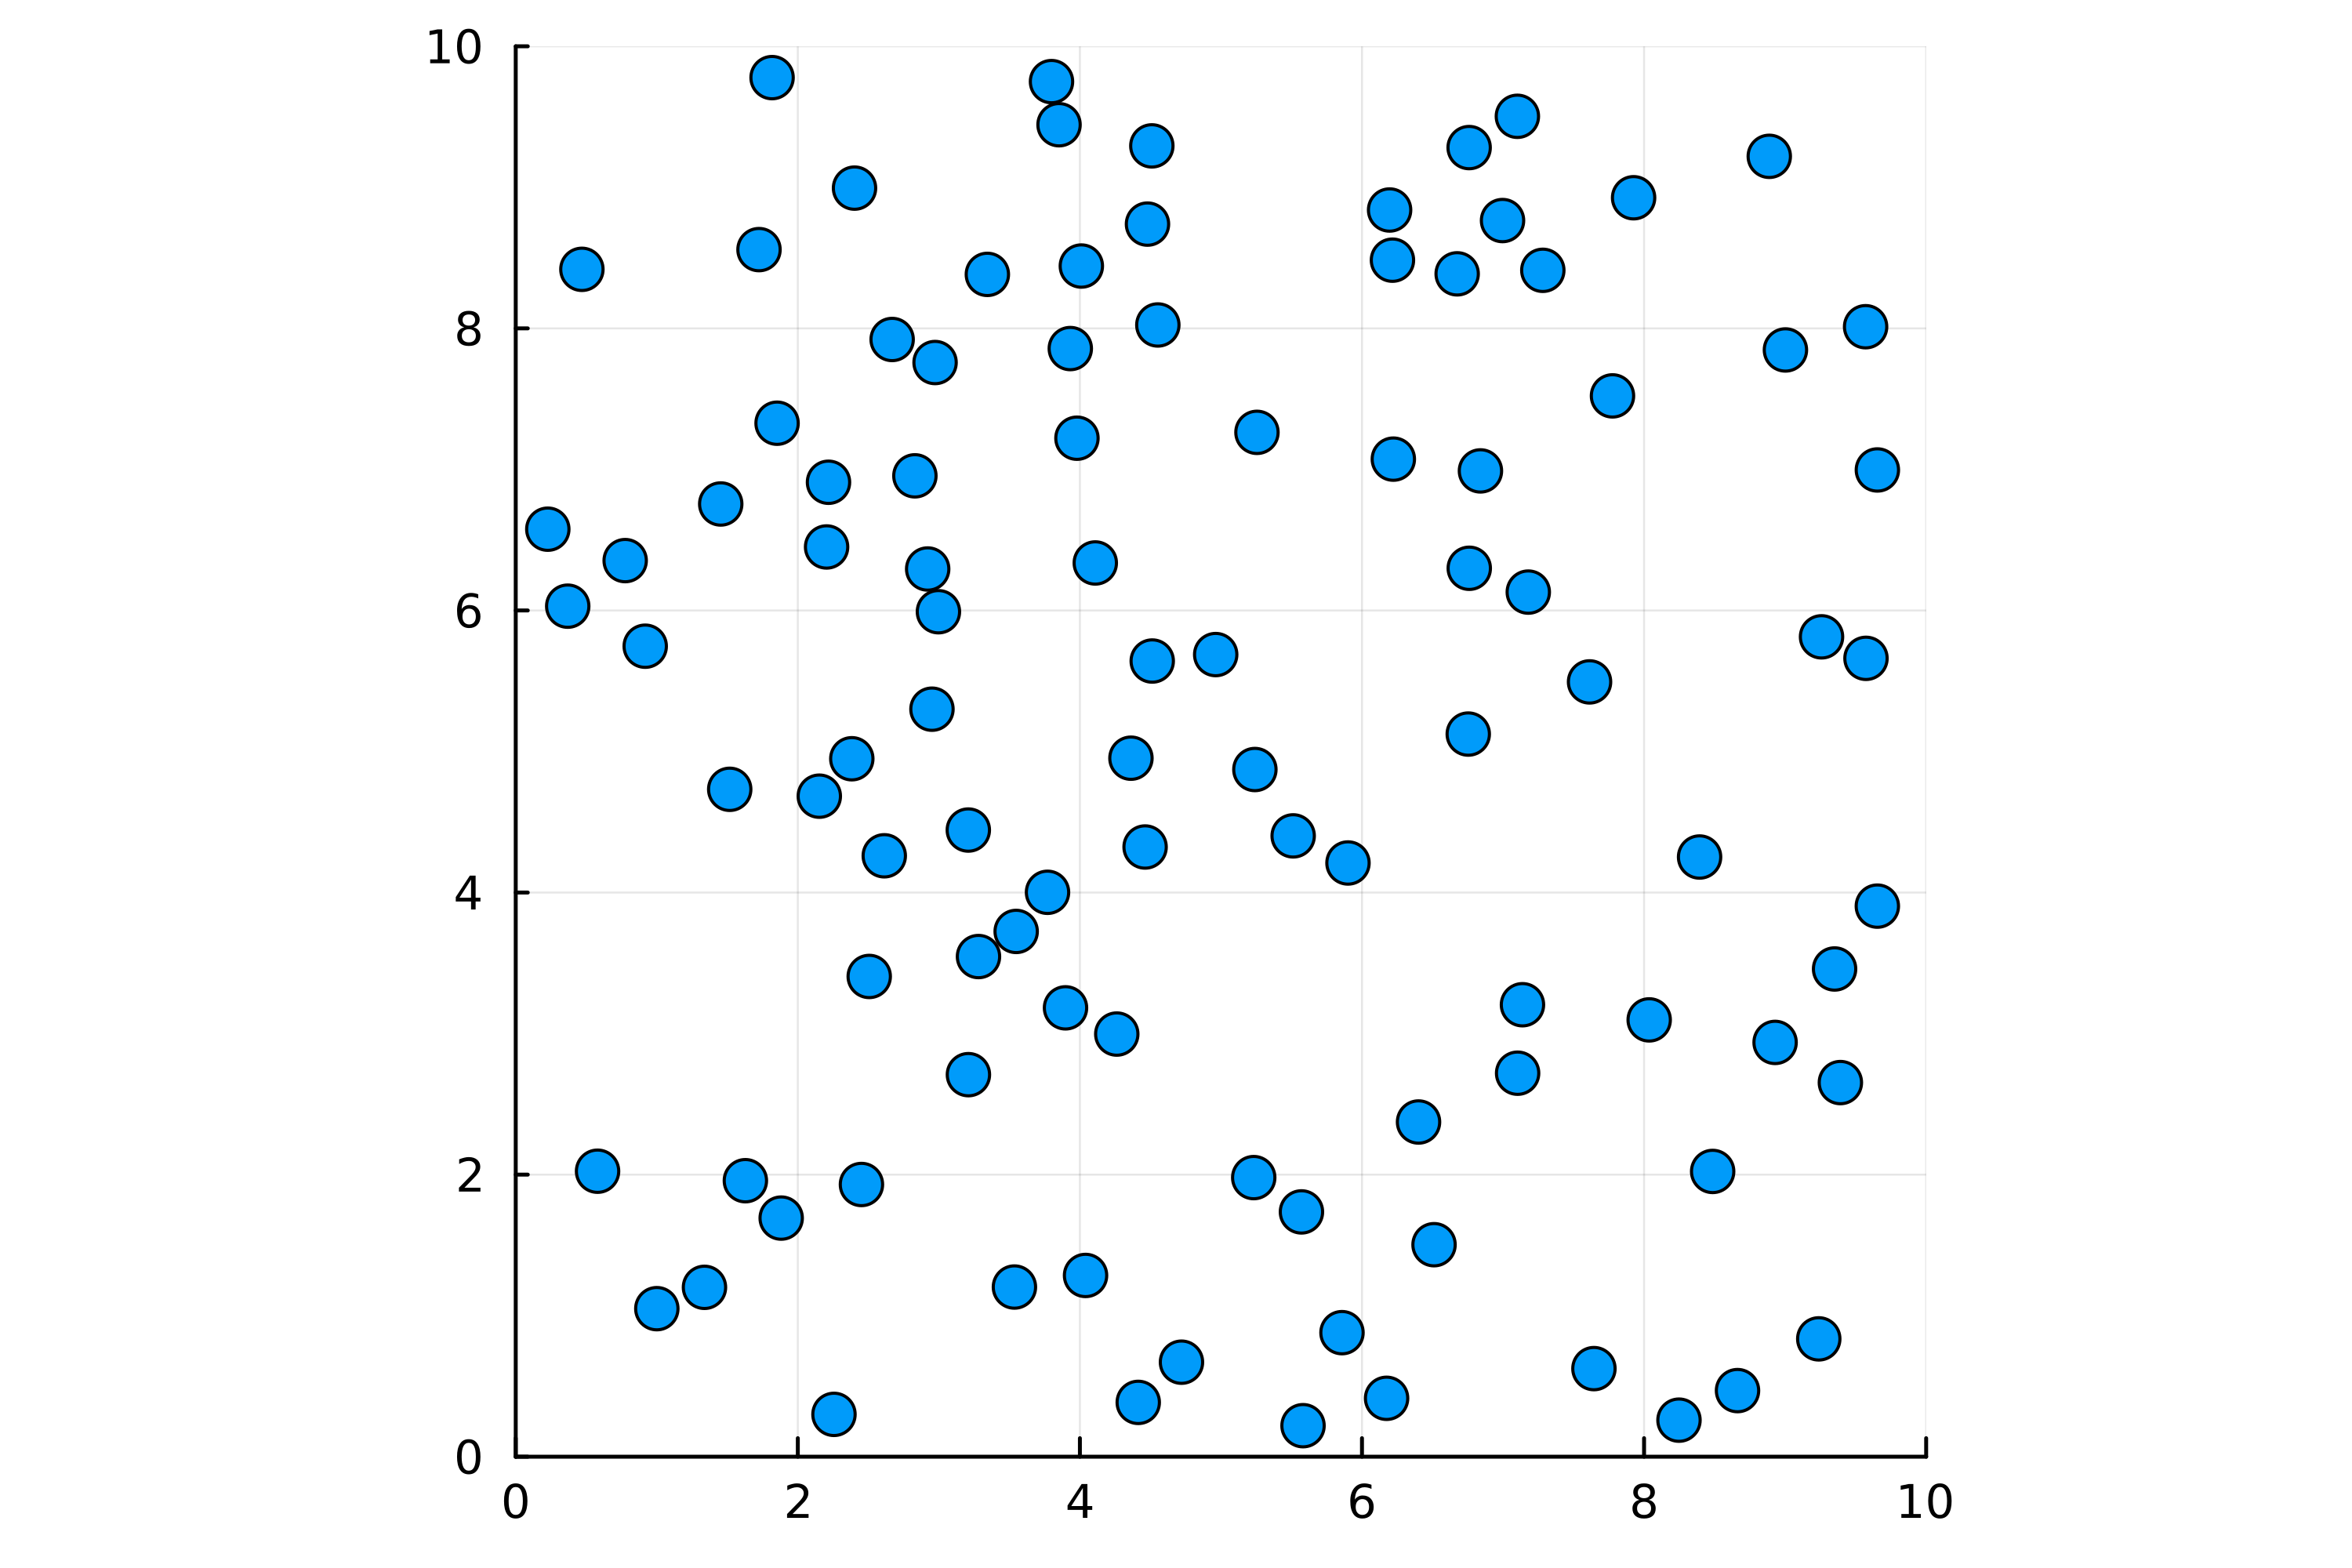
\includegraphics[width=\textwidth]{bachelors-thesis/model_illustrations/SphereModel.png}
		\caption{In contrast to Figure (a), the particles do have a real radius in the sphere models. 
        This causes particle interaction terms as addition in the particle movement, since particles can now collide. 
        The type of interaction terms determines whether it is a hardsphere or softsphere model.   }
	\end{subfigure}
	\hfill
	\begin{subfigure}{0.4\textwidth}
		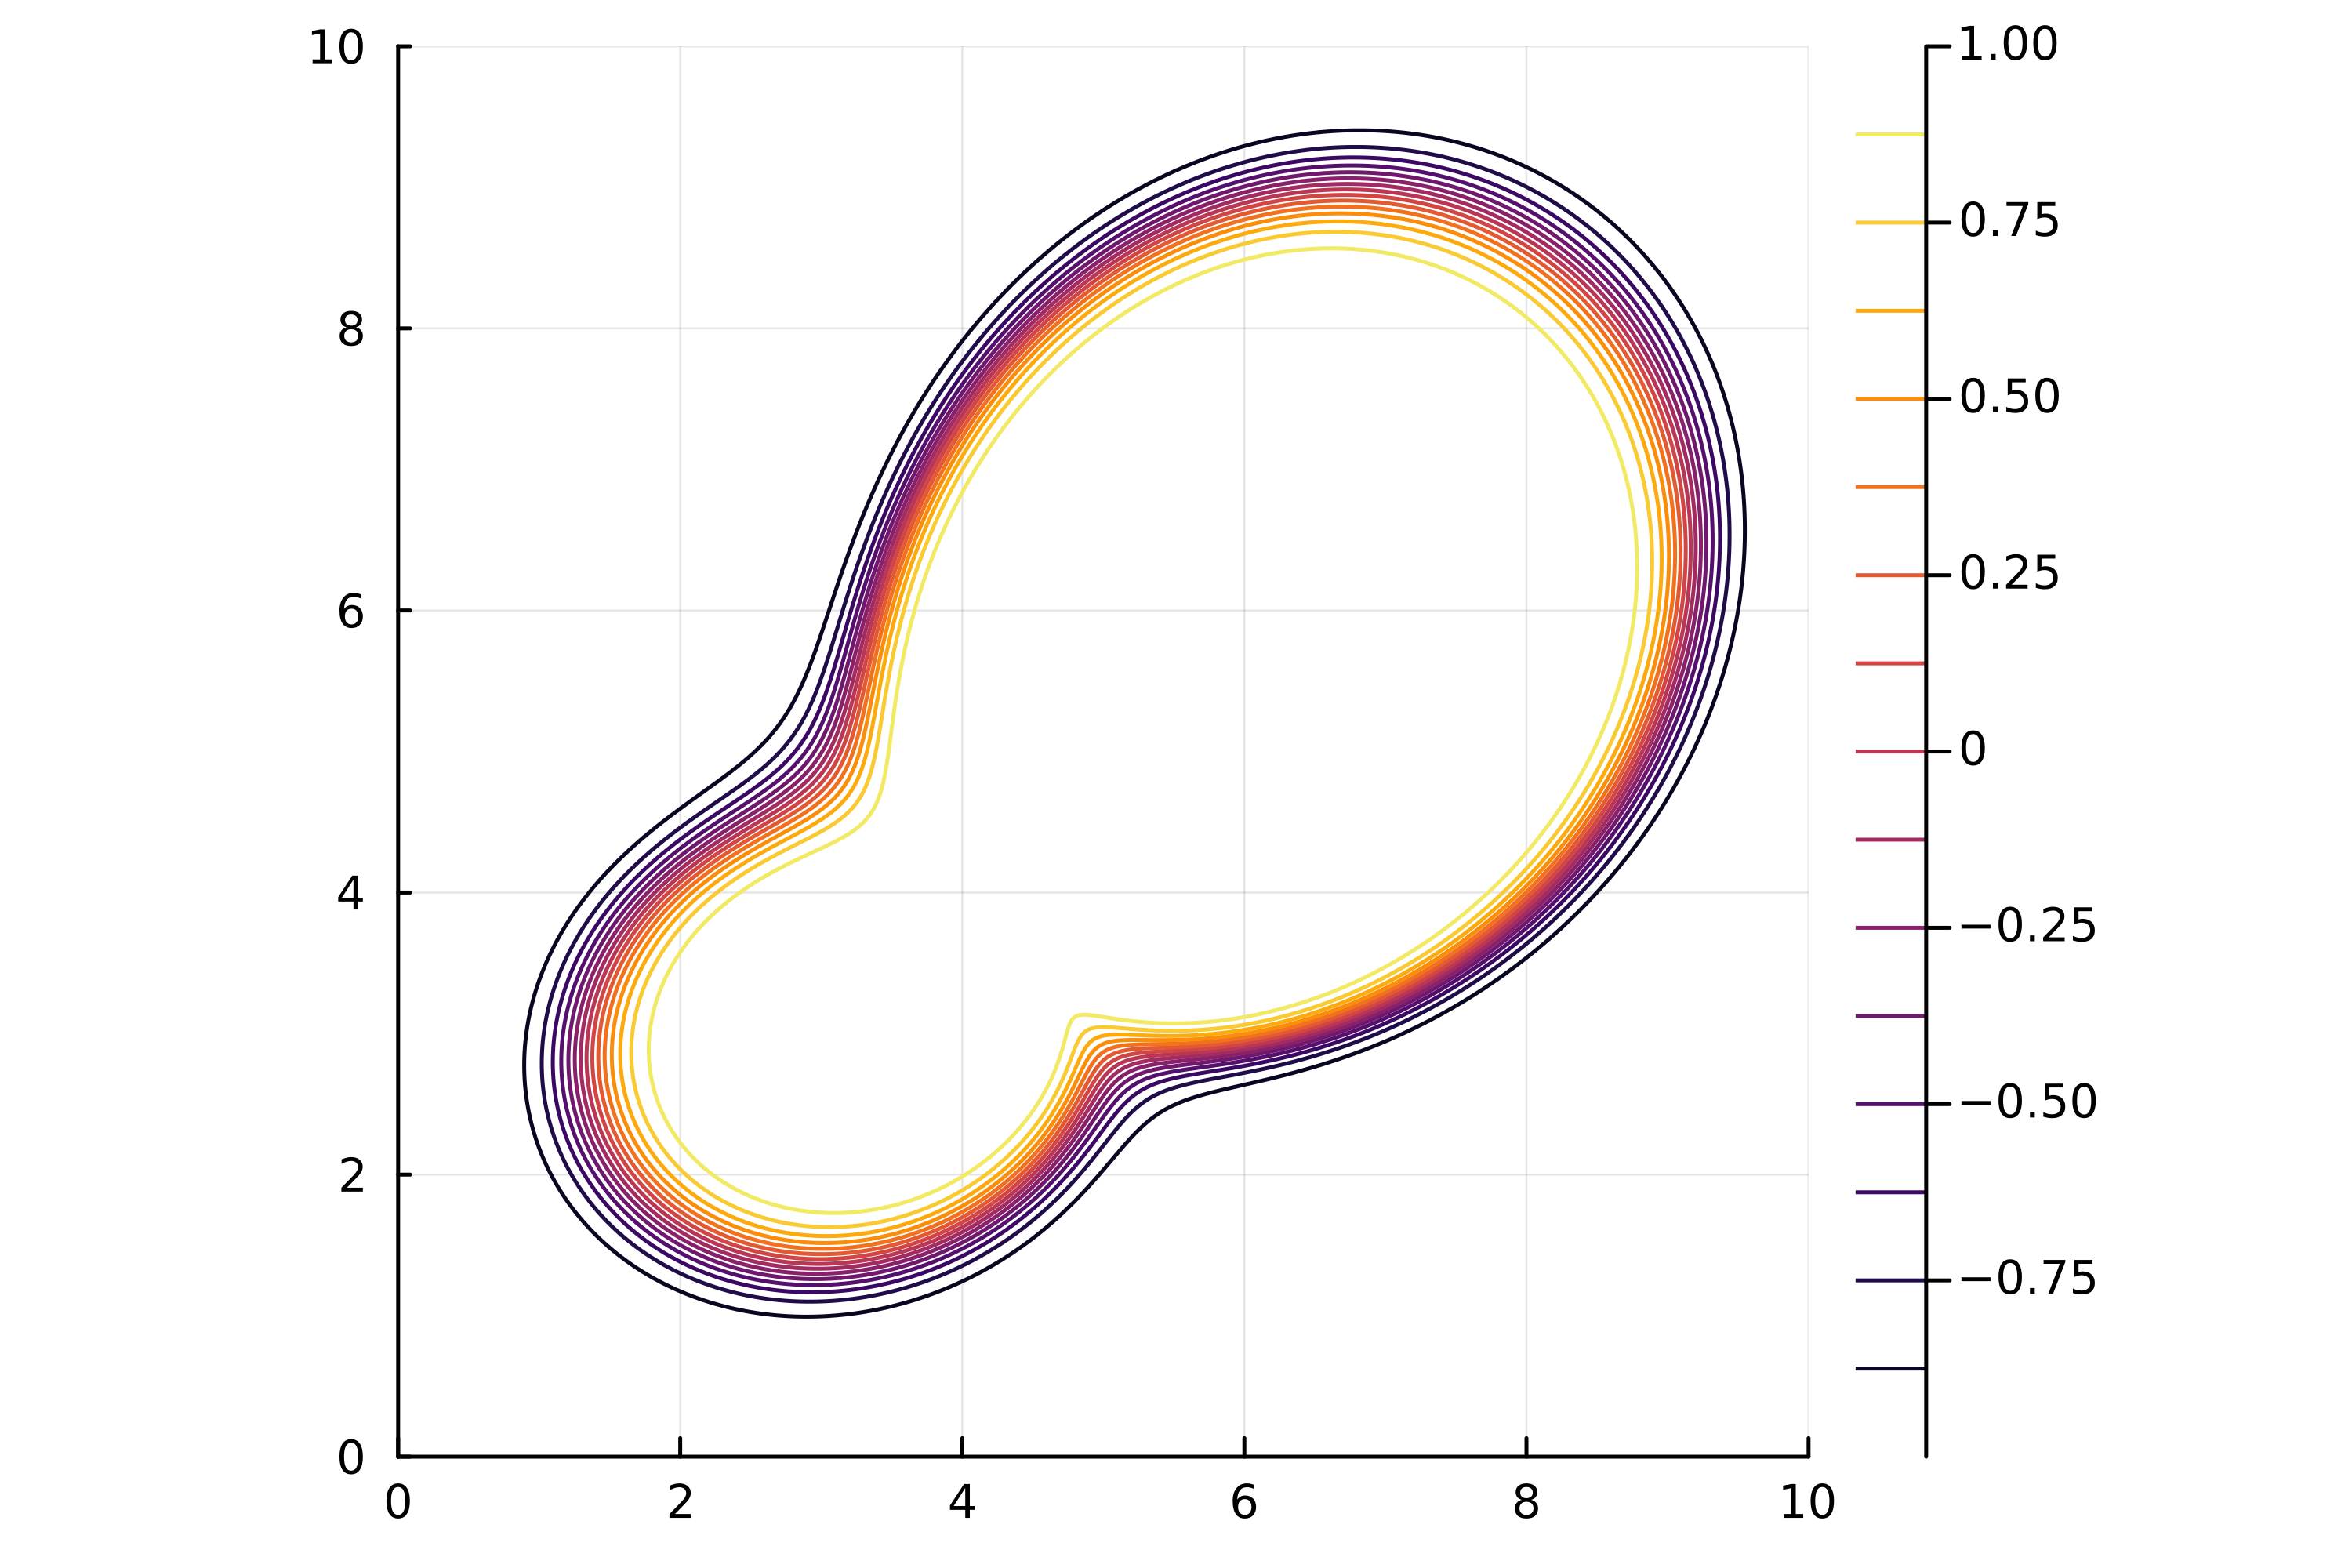
\includegraphics[width=\textwidth]{bachelors-thesis/model_illustrations/PhaseFieldModel.png}
		\caption{A contour plot of a phase field variable $\phi$ illustrates how cells can be modeled through phase field models. 
        The cell's inside is the area where $\phi > 0$. 
        The cell wall sits on the red line where $\phi = 0$. 
        The outer lines display the smooth transition to the outside. }
	\end{subfigure}\hfill
	\begin{subfigure}{0.4\textwidth}
		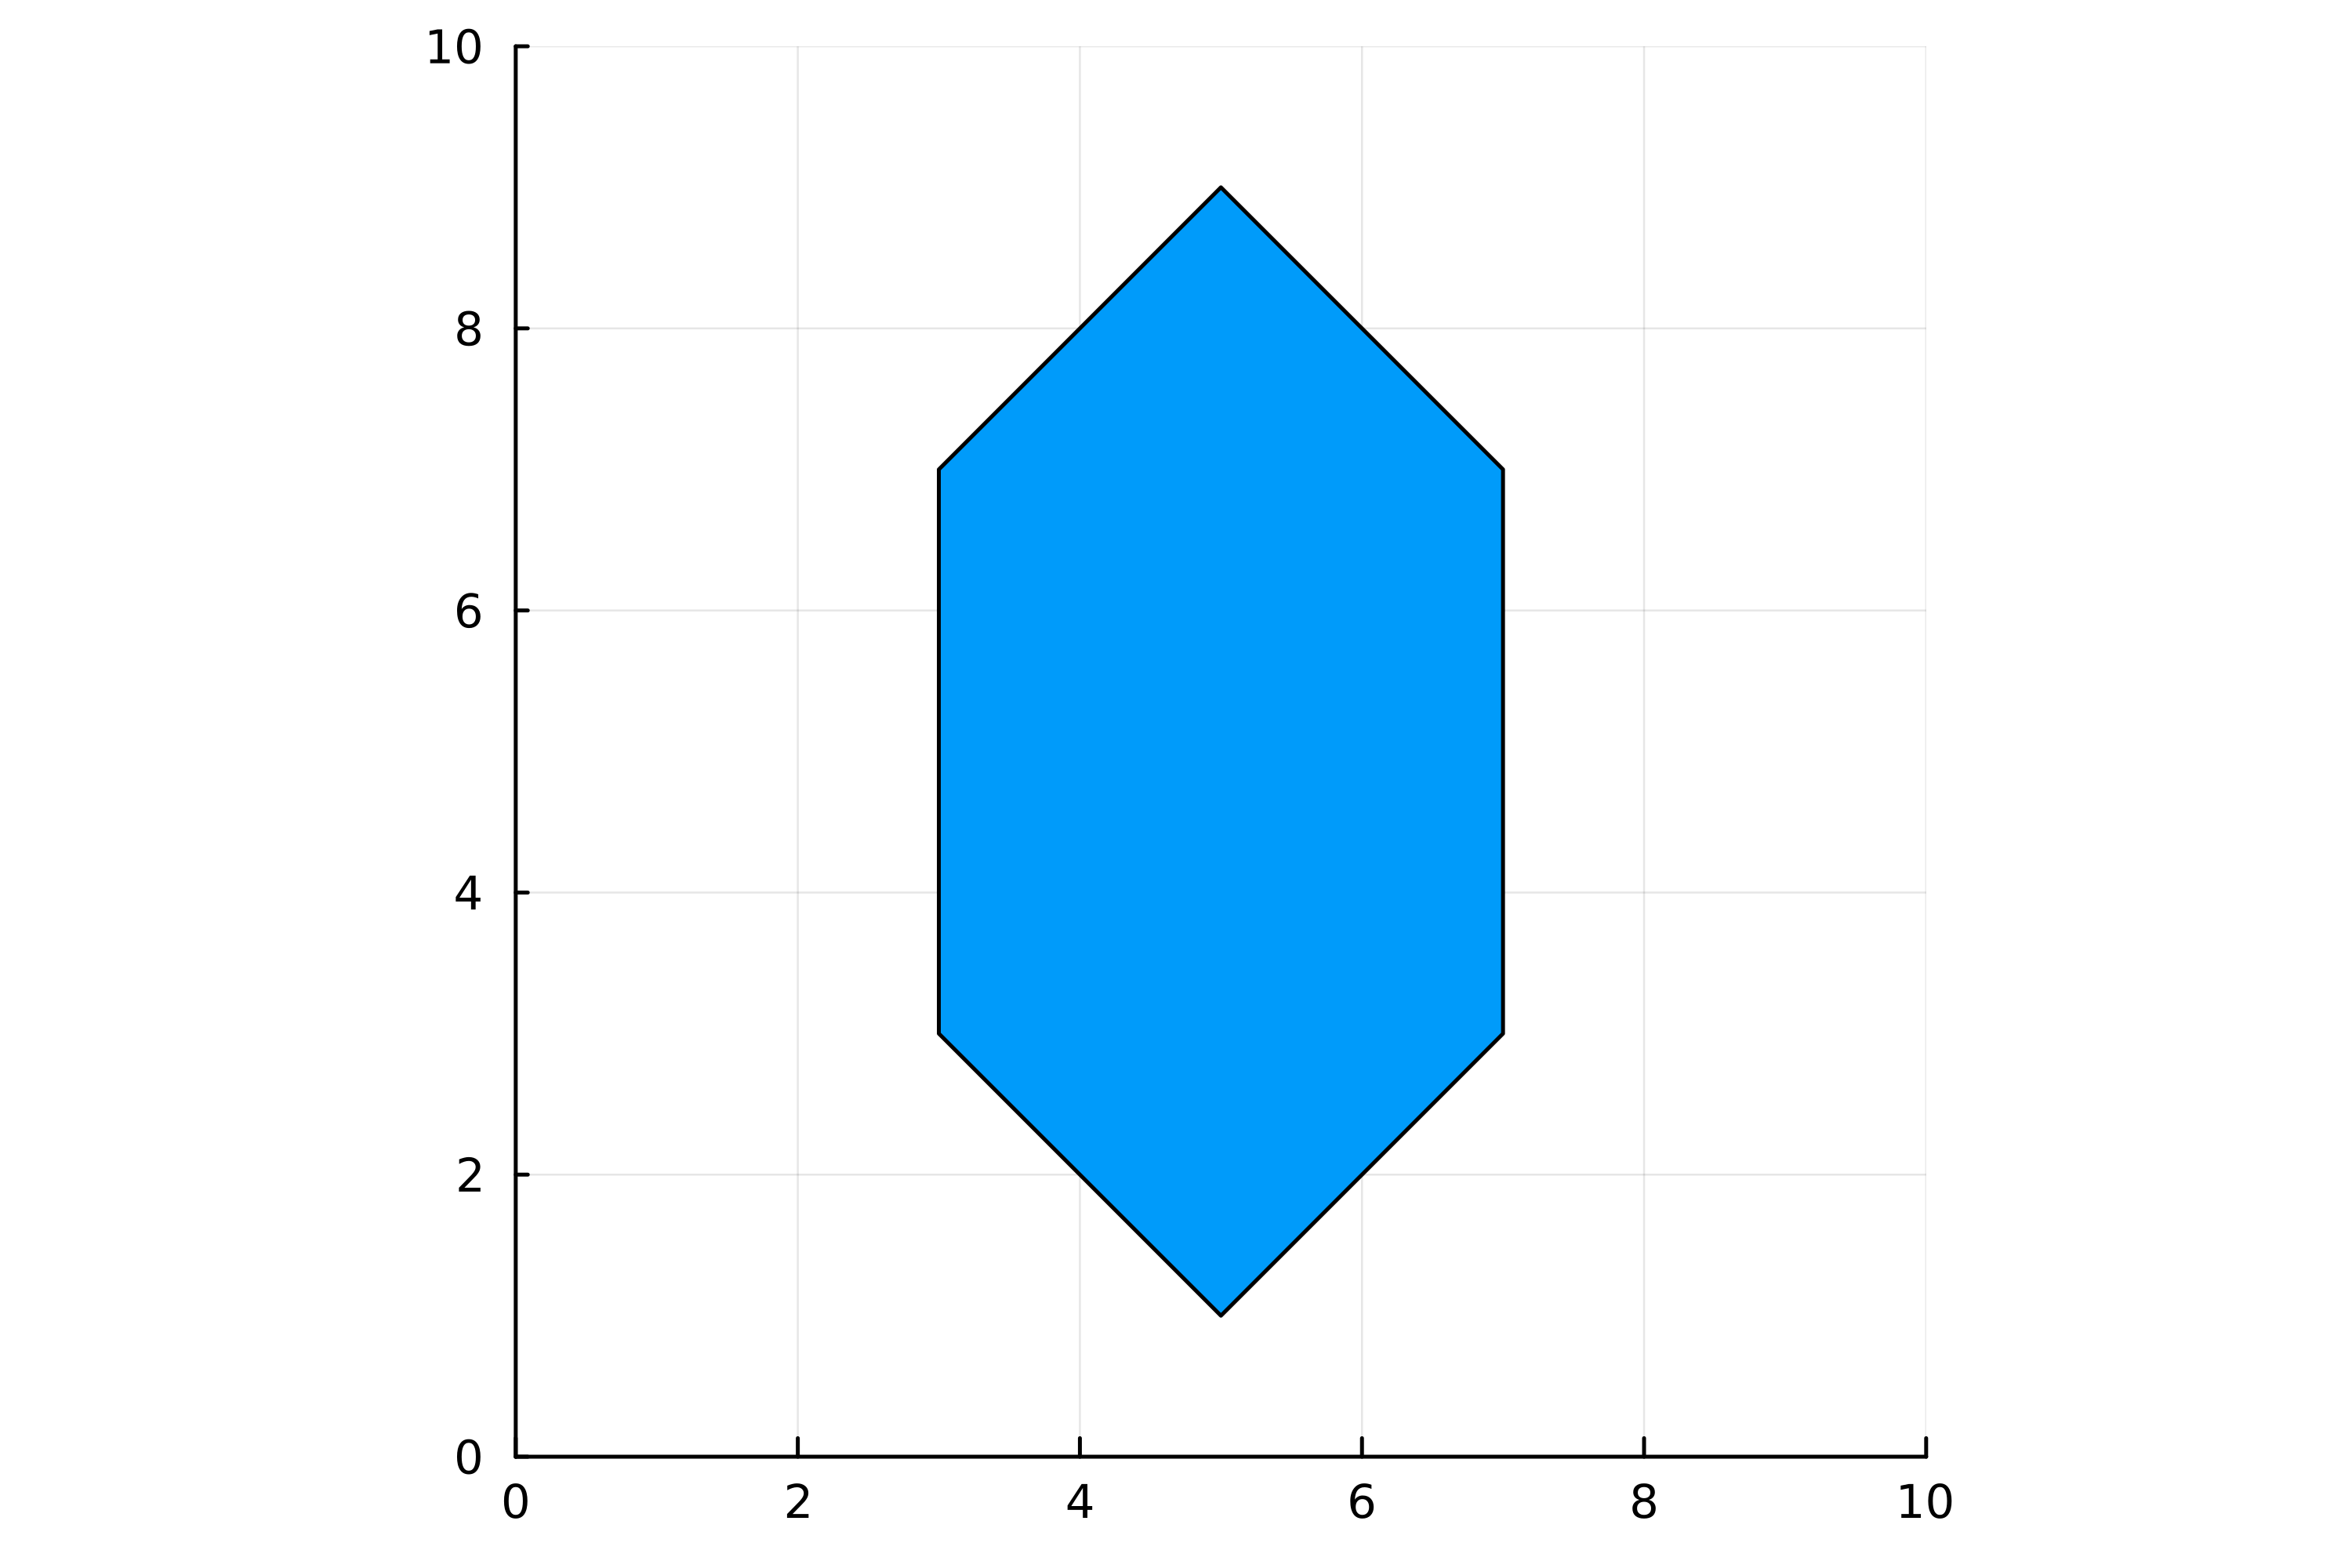
\includegraphics[width=\textwidth]{bachelors-thesis/model_illustrations/VertexModel.png}
		\caption{Another possibility to model cell forms are Vertex models. 
        An example of this is shown here. 
        This cell has six vertices. 
        In order to model cell deformations, one can define forces that act on each vertex separately and thus cause them to move in an according direction. }
	\end{subfigure}
	\caption{ To illustrate the models from the introduction, we can see a corresponding plot for each model. 
    In (a) and (b) the focus is more on the density distribution of the particles in $\Omega$. 
    The amount of particles is $N = 100$. The remaining sub figures (c) and (d) are concerned with the representation of cell shapes. 
    In all sub figures, the axes denote the spatial $x$ and $y$ coordinates. } 
	\label{fig:model_illus}
\end{figure}
In this thesis, we aim to derive forces that can be applied to our cell model and affect the diffusion behavior of the cell system, similar to the forces studied in~\cite{Bruna2012} and~\cite{Bruna2017}. \\

% transition to phase field models 
While these models are powerful, they are limited to spherical particles and do not account for the complex shapes and deformations observed in biological cells.  \\


% phase field model
\textbf{Phase field model} \\

% intro phase field model: 
- A new cell model approach is now considered. 
- The principle of phase field models shares conceptual similarities with the soft-sphere model of Bruna, Chapman, and Robinson~\cite{BCR17} in that both incorporate cell-cell interactions through a continuous, repulsive energy term that prevents interpenetration. 
- In both frameworks, the interaction is mediated by a smooth, short-range potential (via the diffuse interface in the phase field model and via a potential 
u in the soft-sphere model), leading to a physically realistic representation of cell crowding. 
However, the phase field model differs fundamentally in its approach: it is a continuum differential equations-based model that explicitly represents cell shape and internal structure through a phase field variable $\phi_i$, allowing for complex deformations, topological changes, and geometric coupling to surface curvature. 
- In both models, cell-cell interactions are mediated through a continuous, short-range potential that prevents interpenetration while allowing for deformations, leading to a smooth transition between overlapping and non-overlapping states. 
- The soft-sphere model derives its interaction term from a potential energy function $u(\|\vec{x}_i - \vec{x}_j\|_2)$, which results in a nonlinear diffusion equation with a density-dependent diffusion coefficient. Similarly, the phase field model uses a diffuse interface representation where the interaction energy arises from a non-local term in the free energy, effectively generating a repulsive force between cells that scales with local cell density. 
- These shared mathematical structures and physical principles — namely, gradient flow dynamics, continuous interactions, and density-dependent diffusion — highlight the conceptual and formal parallels between the phase field approach and the soft-sphere model. \\
- While the phase field model shares core principles with the soft-sphere model—such as continuous interactions and density-dependent diffusion—it differs significantly from both the soft-sphere and hard-sphere models in its representation and physical implementation. 
Unlike the soft-sphere model, which treats cells as point particles with a smooth interaction potential, the phase field model explicitly represents cells as extended, diffuse regions with a continuous internal structure defined by the phase field variable $\phi_i$. \\

This allows for natural handling of complex cell shapes, topological changes (such as cell division or fusion), and the coupling of cell mechanics to geometric curvature through extrinsic curvature terms in the free energy. 
- the phase field model resolves overlaps through gradual, continuous deformation of cell interfaces, avoiding discontinuities in dynamics. 
- Both frameworks are based on a variational principle, where cell dynamics are governed by a gradient flow of a free energy functional that incorporates shape preservation, cell-cell interactions, and the physical constraints of the system. 
- contrasts to the sphere models are: 
- the hard-sphere model enforces rigid, non-deformable boundaries via reflective boundary conditions at a fixed distance, resulting in abrupt, instantaneous collisions without shape deformation.  The phase field model, by contrast, resolves overlaps through gradual, continuous deformation of cell interfaces, avoiding the discontinuities inherent in hard-sphere dynamics. \\

Phase field variables represent cells as smooth functions $\phi_i(\vec{x}, t) \in [-1, 1]$, with $\phi_i > 0$ in the cell interior and $\phi_i <0$ in the exterior. 
The cell wall is denoted by values of $\phi_i = 0$. \\
The dynamics of $\phi_i$ are governed by a gradient flow of a free energy functional:
\begin{align*}
	\frac{\partial \phi_i}{\partial t} + v_0 (\vec{v}_i \cdot \nabla_{\vec{x}} \phi_i) = \Delta_{\vec{x}} \frac{\delta F}{\delta \phi_i}, \qquad 1 \leq i \leq N 
\end{align*}
where $\vec{v}_i$ is a vector field used to incorporate activity, with a self propulsion strength $v_0$, $F$ is a free energy, and $\dfrac{\delta F}{\delta \phi_i}$ denotes the first variation.\\
The free energy $F$ arises from a sum of different energies, 
\begin{align*}
	F = F_{CH} + F_{INT} + F_{M}. \\
\end{align*}
The first energy is a Cahn-Hilliard energy and could look like in~\cite{wenzel2021}
\begin{align*} 
	F_{CH} = \sum\limits_{i=1}^N \int_{\Omega} \dfrac{1}{Ca} \left( \dfrac{\epsilon}{2} \norm[\nabla_{\vec{x}} \phi_i]^2 + \dfrac{1}{\epsilon} W(\phi_i) \right) d\vec{x},
\end{align*}
$\epsilon$ is a small parameter related to the interface thickness, and $Ca$ is a capillary number that scales the relative importance of surface tension.
The term $\norm[\nabla_{\vec{x}} \phi_i]^2$ penalises a long cell wall, as $\nabla_{\vec{x}} \phi_i \neq 0$ only at the cell wall.
$W(\phi_i) = \dfrac{1}{4} (\phi_i^2 - 1)^2$ is a double-well potential. 
This energy ensures that each $\phi_i$ maintains a stable interface of $[-1,1]$.  \\ 
The second energy term $F_{INT}$ models cell-cell interactions and could be defined as in~\cite{wenzel2021}
\begin{align*}
	F_{INT} = \sum\limits_{i=1}^N \frac{1}{Ca} \int_{\Omega} B(\phi_i) \sum\limits_{j \neq i} w(d_j) \: d\vec{x},
\end{align*}
where 
\[B(\phi_i) = \dfrac{3}{4\sqrt{2}\epsilon} (\phi_i^2 - 1)^2\]
is an approximation of the delta function of the cell boundary that is non-zero only at the cell wall.
The sum in the integral accounts for the interaction with all other cells $j \neq i$ through a short-range potential $w(d_j)$, where $d_j$ is the signed distance function to the cell boundary of cell $j$.  

The third energy term $F_M$ differs for different models and incorporates additional mechanical properties of the cells, such as area conservation or bending energy.% phase field comparison paper:

- In \cite{wenzel2021}, the authors focussed on the influence of microscopic details to incorporate active forces on emerging phenomena.
The models are based on cell deformations and cell-cell interactions and we investigate 
- We compare four different approaches, one in which the activity is determined by a random orientation, one where the activity is related to the deformation of
the cells, and two models with subcellular details to resolve the mechanochemical interactions underlying cell
migration.
- The models are compared with respect to generic features, such as coordination number distribution,
cell shape variability, emerging nematic properties, as well as vorticity correlations and flow patterns in large
confluent monolayers and confinements. 
- The random model determines the direction of motion on the single cell level by a stochastic process
- elongation model aligns the direction of motion with the long axis of the cell
- polar and a nematic model, which use subcellular details to determine strength and direction of motion on a single cell level.

- The goal of this paper is a systematic comparison of these approaches and their linkage with statistical observables of experiments to provide a route towards predictive simulations of patterns and correlations in cell colonies. After introducing the multiphase field models, discussing microscopic differences, and briefly describing the numerical approach enabling large-scale simulations, we address coordination number distribution, analyze statistics on shape variability of the cells and the ratio of multicellular rosettes, velocity distributions of emerging topological defects, their stress fields, as well as defect density and creation rates
- All results are compared with experimental data for a large variety of cell cultures. The appearing qualitative differences of the models show the importance of microscopic details.

\begin{table*}[h!]
\centering
\begin{tabular}{>{\scriptsize}l >{\small}c  >{\small}c  >{\small}c  >{\small}c} % l = left aligned, c = centered, r = right aligned
\hline
characteristic & Random & Elongation & Polar & Nematic \\ 
\midrule
Coordination number distribution & ($\checkmark$) & ($\checkmark$) & ($\checkmark$) & ($\checkmark$) \\[0.5em]
Shape variability & ($\checkmark$) & $\checkmark$ & $\checkmark$ & ($\checkmark$) \\[0.5em]
Rosette ratio & \multicolumn{4}{>{\small}c}{Differences between models} \\[0.5em]
Velocity distribution of topological defects & \multicolumn{4}{>{\small}c}{Differences between models} \\[0.5em]
Correlation between direction of motion and orientation of defect & $\boldsymbol{\times}$ & $\checkmark$ & $\checkmark$ & ($\checkmark$) \\[0.5em]
Elastic property of + 12 defect & $\boldsymbol{\times}$ & Extensile & Contractile & Contractile \\[0.5em]
Active turbulence & ($\checkmark$) & ($\checkmark$) & ($\checkmark$) & ($\checkmark$) \\[0.5em]
Vorticity-vorticity correlation & \multicolumn{4}{>{\small}c}{Similar for all models} \\[0.5em]
Dependency of defect density on activity & Linear & Linear & Linear & Constant \\[0.5em]
Rotational motion in circular confinement & $\boldsymbol{\times}$ & ($\checkmark$) & $\boldsymbol{\times}$ & $\boldsymbol{\times}$ \\[0.5em]

\bottomrule
\end{tabular}
\caption{Comparison of the four different phase field models from~\cite{wenzel2021} with respect to various characteristics observed in experiments. 
A check mark $\checkmark$ indicates observed agreement, $\boldsymbol{\times}$ indicates disagreement and ($\checkmark$) indicates only qualitative agreement with universal feature. 
If experimental data are not available or insufficient for a comparison, only similarities or differences of the models are noted.}
\end{table*}
% phase fields on curved domains 

- it focuses on emergent collective behaviors such as coordinated rotation on curved surfaces, driven by curvature alignment and self-propulsion. 
In contrast to the hard-sphere model, which enforces rigid, instantaneous collisions via reflective boundary conditions, 
These differences make the phase field model particularly suited for studying morphogenesis and tissue mechanics, but it does not yield a macroscopic diffusion equation like those in the soft-sphere or hard-sphere frameworks.
- Furthermore, while the soft-sphere model typically assumes spherical symmetry and isotropic interactions, the phase field model can incorporate anisotropic effects—such as alignment with principal curvature directions—through geometric coupling terms, enabling the simulation of complex collective behaviors like coordinated rotation on curved surfaces. 
These differences make the phase field model more biologically realistic for epithelial tissues, but also more computationally demanding than the simpler point-particle approaches. \\





% vertex based model 
\textbf{Vertex model} \\

% bridge paper:
With precedents in the physics of foams, network models describe epithelial tissues as networks of polygonal cells. Thus, albeit in less detail than lattice and phase-field models, these models still describe subcellular features of cell shape. They encompass two subtypes of models: vertex and Voronoi models.

- In vertex models, the degrees of freedom are the vertices of the polygons.
- Alternatively, the network can be described by the cell centers, and this reduces the number of degrees of freedom. These descriptions are known as Voronoi models because, given the positions of the cell centers, the cell–cell boundaries are delineated by the Voronoi tessellation
- The difference in the number of degrees of freedom has important consequences for the mechanical properties of the network, which may thus differ between vertex and Voronoi models 
- In Voronoi models, the network is dynamic, evolving with each recomputation of the tessellation
- In vertex models, by contrast, network rearrangements entail the appearance and disappearance of vertices, which requires implementing specific rules
% bachelor thesis 
A simpler approach for modeling diverse shapes in cell models is to use a vertex-based model, as used in~\cite{Fletcher14}. 
Vertex models are a valuable tool in computational biology and biophysics for studying the biomechanics and behavior of cells and tissues. \\
In a vertex model of a cell, the cell's outline or boundary is approximated as a polygon, with the vertices of this polygon representing discrete points along the cell's boundary. 
Movements or transformations of the cell are given by forces that are applied on each vertex individually. \\
The cell dynamic in a vertex model is given by the equation
\begin{align}
	\eta \dfrac{d \vec{x}_i}{dt} = F_i, \qquad 1 \leq i \leq N \label{eq:vertexmodel}, 
\end{align}
where $\eta$ is a scaling factor and $F_i$ is the total force acting on $\vec{x}_i$. \\
Like in the phase field model, $F_i$ is a sum of different forces that define the cell behavior, such as the cell flexibility or the interaction with other cells. \\
Our new cell model shall be able to represent a wide range of shapes, similar to the phase field model in~\cite{Happel2023} and the vertex model in~\cite{Fletcher14}. \\



% transition to our model:
\textbf{Discrete form model} \\ 
%%% TODO: explain what was done in bachelor thesis 
The DF model shares several key features with the referenced cell models. 
All frameworks after the point particles account for excluded-volume effects, which prevent cell overlap and lead to enhanced diffusion and non-trivial collective behavior. 
The dynamics in each model are governed by gradient flows of energy functionals, ensuring that the system evolves toward lower-energy configurations. 
Furthermore, stochastic motion—modeled as Brownian motion—is included in all approaches to capture thermal fluctuations. 
These shared principles provide a strong foundation for comparing our model to established frameworks.
Like the vertex model of Fletcher et al.~\cite{Fletcher14}, our cells are represented as polygons with discrete vertices, and their dynamics are governed by forces derived from energy gradients. 
However, unlike the standard vertex model, our framework explicitly incorporates a **hardness parameter $h \in [0,1]$** that allows for a continuous transition from rigid hard-sphere behavior ($h=1$) to fully deformable cell dynamics ($h=0$).
In this thesis, we derive and study a non-confluent DF model that systematically investigates how cellular deformability—controlled by the hardness parameter $h$—influences the overall diffusivity of the cell system. 
By connecting our model to the established frameworks of Bruna and Chapman~\cite{Bruna2012, Bruna2017} and Happel and Voigt~\cite{Happel2023}, we provide a unified perspective on cell dynamics that spans from rigid to deformable regimes.

%%% TODO: work in missing papers 
%%% TODO: tell what happens in the following chapters 

